% !TeX root = ../main.tex
% Add the above to each chapter to make compiling the PDF easier in some editors.

\chapter{Evaluation}\label{chapter:evaluation}

\section{Statistical Analysis Results}

\begin{center}
\begin{table}[h]
    \centering
    \begin{tabular}{||c||c|c|c|c|c|c|c|c|c||}
    \hline
         Methods & \(\delta_1 \uparrow\)  & \(\delta_2 \uparrow\) & \(\delta_3  \uparrow\)  & REL \(\downarrow\) & RSE \(\downarrow\) & \(\log_{10} \downarrow\) &  RMSE \(\downarrow\) & RMSLE \(\downarrow\) & SiLog \(\downarrow\) \\
    \hline \hline
         3DGS & 0.851 & 0.851 & 0.852 & 0.139 & 0.111 & 0.140 & 0.311 & 0.841 & 77.96\\
         2DGS & 0.855 & 0.855 & 0.855 & 0.131 & 0.107 & 0.139 & 0.311 & 0.838 & 77.50\\
         RaDe & \textbf{0.856} & 0.856 & 0.856 & \textbf{0.128} & 0.106 & 0.138 & 0.310 & 0.837 & 77.34 \\
         GS2M & 0.853 & 0.853 & 0.853 & 0.155 & 0.124 & 0.138 & 0.309 & 0.833 & 77.04 \\
         DA1-s & 0.807 & 0.903 & \textbf{0.957} & 0.143 & \textbf{0.027} & \textbf{0.048} & 0.097 & 0.252 & 24.71\\
         DA1-b & 0.828 & \textbf{0.907} & 0.948 & 0.154 & 0.032 & 0.049 & \textbf{0.095} & \textbf{0.251} & \textbf{24.25} \\
         DA1-l & 0.725 & 0.831 & 0.898 & 0.278 & 0.061 & 0.081 & 0.118 & 0.359 & 33.88 \\
         DA2-s & 0.561 & 0.688 & 0.788 & 0.502 & 0.094 & 0.140 & 0.127 & 0.503 & 43.32  \\
         DA2-b & 0.583 & 0.710 & 0.811 & 0.443 & 0.079 & 0.129 & 0.127 & 0.472 & 41.95\\
         DA2-l & 0.613 & 0.745 & 0.850 & 0.354 & 0.058 & 0.110 & 0.124 & 0.419 & 38.47 \\
         ZoeD & 0.472 & 0.620 & 0.742 & 0.679 & 0.163 & 0.179 & 0.159 & 0.581 & 47.51 \\
    \hline
    \end{tabular}
    \caption{Statistical analysis on GT values}
    \label{tab:stat-analysis}
\end{table}
\end{center}

Table \ref{tab:stat-analysis} shows the result of our statistical analysis on all the MDE and Gaussian Splatting models. From the results above, it can be noted that RaDe-GS seem to have the overall best performance when compared to other Gaussian Splatting models. This seem to be consistent with evaluations done by the authors of RaDe-GS \parencite{radegs}. RaDe-GS is able to produce more detail-sensitive results when compared to 2DGS, GS2Mesh, and the original 3DGS method. Most notably, RaDe-GS is able to achieve the lowest absolute relative error, which means that the RaDe-GS model produce values that most closely resembles the absolute value of the Ground Truth. It also achieves the highest \(\delta_1\) score, which means that out of all of the models, it has the highest percentage of values closely resembling the ground truth.

2DGS, on the other hand, delivers a strong performance and seems to be the overall runner-up amongst the Gaussian Splatting models, although 3DGS and GS2Mesh seem to still perform closely to the other two, with 3DGS performing the worst out of all the Gaussian Splatting models. These findings are consistent with the expected results; 3DGS have a less optimized algorithm, since it is the predecessor of all of the GS models, and GS2Mesh suffer from the same drawbacks as the original 3DGS model, since it employs 3DGS as the core of its pipeline.

When compared to the MDE models, the GS models seem to be competitive. GS models seem to have higher \(\delta_1, \delta_2,\) and \(\delta_3\) values overall, even though the early Depth Anything v1 models seem to be performing well too in this measurement.

Most surprisingly, DepthAnything v1 models seem to be delivering a stronger performance than its successor, the DepthAnything v2, even though DepthAnything v2 is also trained on synthetic data. This may be due to DepthAnything v2 trying to produce more detailed results, which in turn spoiled its evaluation scores since the model being tested is an extremely simple model. ZoeDepth does not seem to be performing well too on the tests. This may be due to ZoeDepth's tendency to add some noise in the background, which might make sense when dealing with real life data, but does not work well when dealing with models with no background.

Overall, the most accurate depth values seem to be generated by the DepthAnything v1 base model, with it having the overall lowest RMSE, RMSLE, and SiLog values and the highest \(\delta_2\) value. The GS models seem to perform poorly on the SiLog evaluation, which mean that the GS models might be consistently off by some factor, even though this factor seem to not be significant when compared to the ground truth value, since the GS models have high threshold accuracy percentages.

\section{Visual Analysis Results}

\begin{figure}[h]
    \centering
    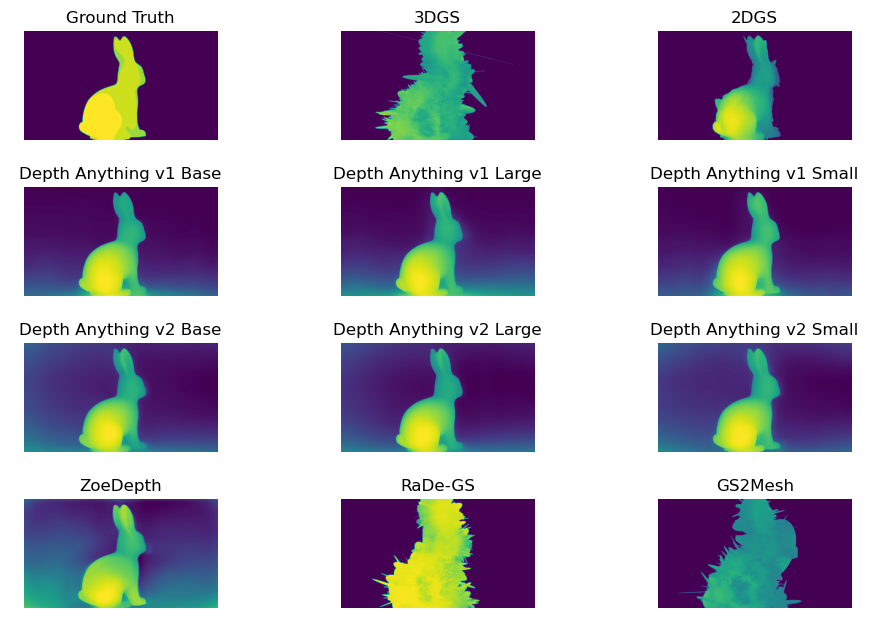
\includegraphics[width=1.0\linewidth]{figures/visual-comparison-1.png}
    \caption{Visual comparison of Chocolate Easter Bunny, facing to the back}
    \label{fig:visual-analysis-1}
\end{figure}

In order to facilitate the visual analysis of the depth maps, some transfer functions to invert the depth maps and to adjust extreme values have been applied. Figure \ref{fig:visual-analysis-1} displays the result of one of the poses used for evaluation, placed side-by-side for ease of viewing.

From the results, we can see that the ground truth image generally possess a very basic form with not much variation in depth values. At a glance, out of all the Gaussian Splatting models, the 2DGS model seem to be performing the best visually, since the splats seem to be smoother and deviate less from the general shape of the object. It seem to also be quite detailed, since the folds of the ears are given different depth values and it is possible to visually tell that these details exist solely by looking at the depth map. The legs and the bumps in the bunny's tail is also expressed nicely in the 2DGS model, and we can tell that the bunny is facing to the back. However, we can also tell that 2DGS tends to apply smoothing to the image; the chocolate bunny that is supposed to be a bit flatter is illustrated as being more curvy and more like a real-life bunny with the 2DGS model. This may be the reason that it performs more poorly in the statistical analysis; the ground truth value demands a flatter distribution when compared to the 2DGS bunny.

In contrast to the 2DGS result, the original 3DGS model seem to be very rough and unrefined; the general shape of the bunny can be seen from the depth image, but details are not clear at all. The bunny also does not appear to be facing the back, but rather it creates the illusion that the bunny is facing to the right instead. Furthermore, the splats are very all over the place and often sticks out at a weird angle. This might be due to the model misclassifying general lighting as object. 

Along with the 3DGS model, the GS2Mesh model also seem to be doing poorly; a weirdly-placed splat can be seen around the head area of the bunny and the details are missing, although overall it seem to have a better overall shape than the 3DGS model. The GS2Mesh result also does not seem to be looking to the back, but rather to the side like its 3DGS counterpart.

RaDe-GS, on the other hand, seem to be performing pretty well; it seems to preserve the flatter values of the original training image better than even the 2DGS result, which may be why it performs the best during the statistical evaluation. Visually, though, it is hard to see that the bunny is facing the back, even though it is still more detailed and value-accurate when compared to 3DGS and GS2Mesh. The RaDe-GS result also has a better overall shape compared to 3DGS and GS2Mesh.

Compared to the GS models, the MDE models tend to produce a very smooth and detailed depth map, since here we do not suffer from having any Gaussians floating around the depth map. However, this also makes them suffer from the same problem that the 2DGS model suffers from: oversmoothing the values is not ideal since the Chocolate Bunny model is flatter in general. When compared to each other, it is clear that the DepthAnything v2 large model offers the most-detailed depth values; the folds of the ears are apparent and the tail of the bunny is sculpted more. However, due to these details, the DepthAnything v2 large performs more poorly in the statistical analysis; the small DepthAnything v1 model tends to provide less details, which mean less oversmoothing happened and the images are flatter in general. In Figure \ref{fig:bunny-comparison}, we highlight the difference in details between the DepthAnything v2 large model and the DepthAnything v1 small model. The red rectangle shows the ear curves, while the blue rectangle shows the oversmoothing problem that the larger models suffer from. Another thing that is detrimental to larger and more recent DepthAnything models is the background; they tend to "bleed", meaning some noise were added into the depth map, while the smaller, older models tend to be less expressive in general.

\begin{figure}[h]
    \centering
    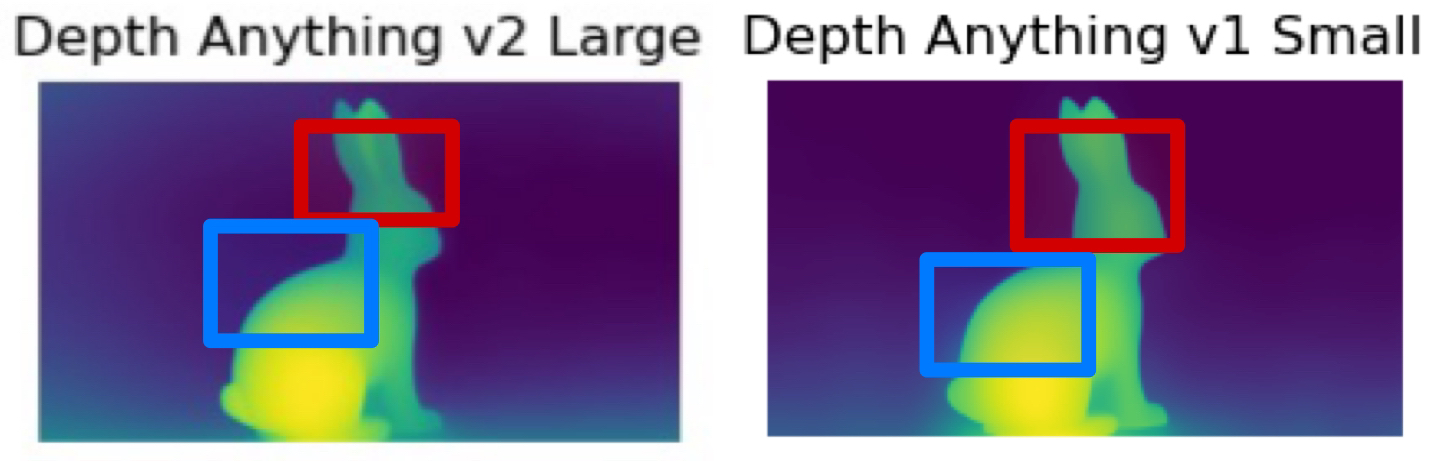
\includegraphics[width=1\linewidth]{figures/bunny-comparison.png}
    \caption{Highlighting discrepancies between DA v2 large model and DA v1 small model}
    \label{fig:bunny-comparison}
\end{figure}

The ZoeDepth model, while offering a pretty detailed depth map, suffers more from this background bleeding problem. We can see that the ZoeDepth background tends to be very noisy in general. While this might have some use in real life datasets, this is, of course, detrimental when dealing with models with no background.

\section{Limitations of Current State-of-Art Methods}

From the results of our analysis, we can see that current state-of-art methods were able to perform well on our simple model. Nonetheless, we acknowledge that there are still some weaknesses to the current models that can be observed from our results. First, MDE models seem to struggle from the background bleeding, since it is not used to dealing with situations that are unrealistic, which is the case in our current model, as it is a synthetic model placed on a completely silent background. In contrast to this, the GS models seem to suffer more from the awkward shape of the Gaussians; they tend to be less smooth than expected, even though the overall shape of the objects seem to be retained well. Due to the density of the Gaussians, GS models often appear much more noisy than they really are, since Gaussians with low opacity still has depth values that needed to be considered for the evaluation.